\documentclass{article}
\usepackage{civ}

\title{CIV102: Quiz 1 \\ Unofficial Solutions}
\author{QiLin Xue}
\date{}
\usepackage{mathrsfs}
\usetikzlibrary{arrows}
\setlength{\parindent}{0cm}
\begin{document}

\maketitle
\section*{2007 Quiz}
\textbf{Q1 Solution:} We know that the Earth has a circumference of $40,000 \text{ km}$ (this was stated in the lecture, where the meter was originally defined as one ten millionth of the distance between the North Pole and equator). There are $360$ degrees and $60$ minutes in a degree, so we have:
\begin{equation}
    1 \text{ nautical mile} = \frac{40,000 \text{ km}}{360\cdot 60} = 1.852 \text{ km}
\end{equation}
It is not exactly clear what the relationship between the measuring period, the speed, and the distances, but we can come up with a procedure to measure the speed of a ship:
\begin{enumerate}
    \item Put down the log and start sailing the ship at a constant velocity, placing down knots every eight fathoms.
    \item At a time $T$, stop and count the number of knots $N$, which is the speed of the ship.
\end{enumerate}
If a ship travels at a speed of one knot, then its speed is $0.5144 \text{ m/s}.$ Then in the measuring period $T$, there would have been exactly one knot tied on it. The total distance it traveled in the measuring period is thus:
\begin{equation}
    \Delta d = 8 \text{ fathoms} \cdot \frac{6 \text{ foot}}{1 \text{ fathom}} \cdot \frac{0.305 \text{ m}}{1 \text{ foot}} = 14.64 \text{ m}
    \label{eq:}
\end{equation}
Therefore, since the speed is constant:
\begin{equation}
    0.5144 \text{ m/s}= \frac{14.64 \text{ m}}{T} \implies T=28.5 \text{ s}
\end{equation}

\textbf{Q2 Solution:}
From energy conservation, we have: $E=mg(fh)$ where \begin{equation}
    fh=0.6\cdot 325 \text{ feet} \times \frac{0.305 \text{ m}}{1 \text{ feet}}=59.475 \text{ m}
    \label{eq:}
\end{equation}
If the mass flow rate is $\dot{m}=\rho\dot{V}$ (kg/s), then we have:
\begin{equation}
    4.3 \times 10^9 \text{ W} = \rho\dot{V}gfh \implies \frac{\Delta V}{\Delta t}=7377 \,\mathrm{m^3/s}
    \label{eq:}
\end{equation}
The volume flow rate that goes over the Falls is thus:
\begin{equation}
    \dot{V} \frac{0.4}{0.6}=4900 \,\mathrm{m^3/s}
    \label{eq:}
\end{equation}

\section*{2009 Quiz}
\subsection*{Version 1}

\subsection*{Version 3}
\textbf{Q2 Solution:} Let the total number of daily travelers be $N$ and the capacity be $c$. Let the mass of each person be $m$ and the vehicle weight be $W$. Let the fuel consumption be $f$, the distance traveled be $D$ and the fuel cost be $C$. Then, the total cost is given by:
\begin{equation}
    \text{cost} = \text{(number of vehicles)} \times \text{(mass per vehicle)} \times \text{(liters of fuel per kilogram per meter)} \times \text{(distance)} \times \text{(fuel cost per liter)}
    \label{eq:}
\end{equation}
The number of vehicles is given by $\lceil\frac{N}{c}\rceil$ and the mass of the vehicle is given by: $$cm+W/g+V_\text{fuel}\rho_\text{fuel}$$
We shall assume that the mass of the fuel is negligible, though we will revisit this if two vehicles result in very similar costs at the end. Thus our equation is:
\begin{equation}
    \text{cost} = \left\lceil\frac{N}{c}\right\rceil(cm+W/g)fDC
    \label{eq:}
\end{equation}
The best technology gives me a cost of $\$5142$ per day (bus), while the worst technology gives me a cost of $\$43416$ per day (car), so the answer for part (a) is $\boxed{11.8\%}$.

For part (b), we count the number of operating days per year. There are on average $365 \cdot \frac{5}{7}$ days per year, so the operating cost per year is: $\boxed{\$ 1,340,000}$.
\section*{2011 Quiz}
\subsection*{Version 1}
\textbf{Q1 Solution:} We will assume that the system reaches steady state where the mercury is originally at a height of $T_0=2^\circ \text{ C}$ and is now at a height of $T_1=100^\circ \text{ C}$. We have:
\begin{equation}
    \Delta V = \beta V \Delta T
    \label{eq:}
\end{equation}
where $\beta$ is the coefficient of thermal expansion. I measured the ratio of the inner radius of the tube to the inner radius of the spherical cavity as: $1:6.4$ so the inner radius of the cylinder is $r=0.078125 \text{ cm}$. Thus, if the mercury goes to a height $h$, then the total volume is:
\begin{equation}
    V=\frac{4}{3}\pi R^3 + \pi r^2 h
    \label{eq:}
\end{equation}
and
\begin{equation}
    \Delta V=\pi r^2 \Delta h
    \label{eq:}
\end{equation}
Thus:
\begin{equation}
    \pi r^2 \Delta h=\beta\left(\frac{4}{3}\pi R^3 + \pi r^2 h_0\right)\Delta T
    \label{eq:}
\end{equation}
I measured $h_0=0.594 \text{ cm}$ and plugging in numbers gives me $\Delta h=3.37 \text{ mm}$.

\textbf{Q2 Solution:}Let us assume that Tasmania is a perfect isosceles trapezoid:
\begin{center}
    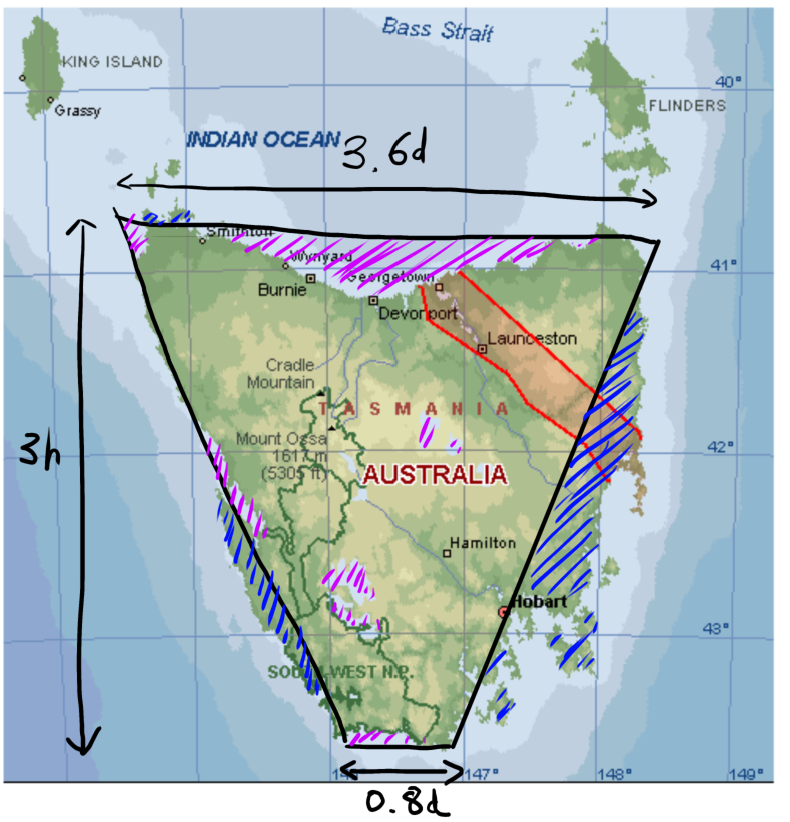
\includegraphics[width=0.5\linewidth]{2011-3-2-S.png}
\end{center}
The justification is that a trapezoid can be picked such that the area of land outside the region is equal to the area of water inside the region approximately. The separation between each latitude line is:
\begin{equation}
    h=\frac{20,000 \text{ km}}{180 \text{ lines}}=111.1 \text{ km}
    \label{eq:}
\end{equation}
and are equally spaced independent of latitude. Longitude lines however, are not equally spaced. At the equator $d=h$ but at a latitude of $42^\circ$, which is $\frac{42}{90}\approx 47\%$ of the way down from the equator to the South pole (where the distance between longitudes is zero), the distance between each longitude line (assuming the distance decreases linearly) is $d=0.47h=52.217 \text{ km}$. The rea of the trapezoid is thus:
\begin{equation}
    A = \frac{1}{2}(0.8d+3.6d)3h=38300 \text{ km}^2
    \label{eq:}
\end{equation}

\end{document}